\chapter{Diseño e implementación} % Main chapter title

En este capítulo se describen las soluciones planteadas al problema resuelto en este trabajo.

%----------------------------------------------------------------------------------------
%	SECTION 1
%----------------------------------------------------------------------------------------
\section{Arquitectura del sistema}

En la figura \ref{fig:arqSistema} se puede observar un esquema simple del sistema, donde se tiene:

\begin{itemize}
	\item Nodos sensores.
	\item Nodo central.
	\item Aplicacion web progresiva.
	\item Broker.
	\item Servidor IoT.
\end{itemize}

\begin{figure}[H]
\centering 
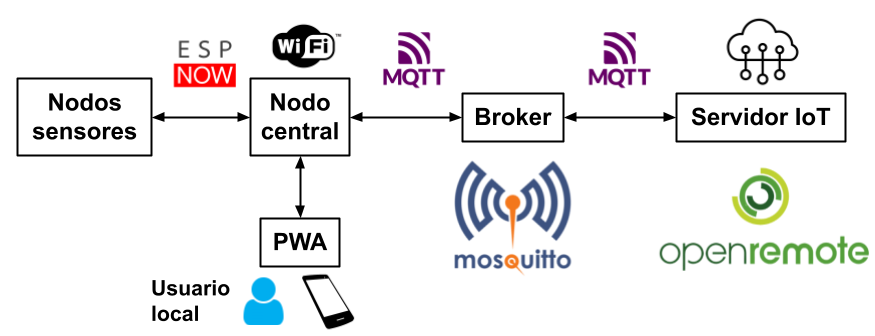
\includegraphics[width=1\textwidth]{./Figures/arq_sistema.png}
\caption{Esquema del sistema.}
\label{fig:arqSistema}
\end{figure}

En esta sección se describen los principales módulos que conforman el sistema, detallando su función y cómo interactúan entre sí.

\subsection{Nodos sensores} 

Están conformados por un módulo ESP32-C3 y un sensor. Esta es la capa de percepción, ya que los nodos son responsables de captar la información del entorno. Los datos recopilados son enviados al nodo central (gateway) a través del protocolo de comunicación ESP-NOW. En este contexto, también se incluye un módulo específico para gestionar los relés, cuyo estado puede ser consultado y modificado, por lo que se establece una \textit{comunicación bidireccional} con el \textit{gateway}. Sin embargo, en el caso de los sensores, la \textit{comunicación es unidireccional}, ya que solo envían datos.

\subsection{Nodo central}

Como se mencionó, este nodo se comunica con los sensores a través de ESP-NOW. Actúa como la capa de transporte, encargándose de transferir los datos capturados por la capa de percepción. Además, el \textit{gateway} integra una interfaz web embebida para visualizar los datos de los sensores y el estado de los relés. Esta interfaz está implementada utilizando un socket y, en caso de ausencia de conexión a internet, genera un \textit{Access Point} (AP) local al cual el usuario puede conectarse para monitorear el estado del invernadero. El nodo central se conecta a internet mediante Wi-Fi para enviar los datos a un \textit{broker} MQTT (Mosquitto), empleando certificados TLS para asegurar la transmisión.

\subsection{Servidor IoT}

Este componente corresponde a la capa de procesamiento, donde se almacenan, analizan y gestionan los datos enviados desde el nodo central. Para esta función, se utilizará \textit{OpenRemote} como plataforma de servidor IoT, la cual facilita la integración de dispositivos y la gestión de datos. El servidor se conecta al \textit{broker} MQTT para recibir la información de los sensores y los relés.
Además de almacenar y visualizar los datos en tiempo real, el servidor permite generar informes, configurar alertas y ejecutar acciones automatizadas basadas en reglas predefinidas, como la activación de relés o notificaciones ante condiciones anómalas.



%----------------------------------------------------------------------------------------
\section{Desarrollo del firmware}

El firmware del trabajo fue desarrollado utilizando el lenguaje de programación python, específicamente bajo el \textit{framework} micropython. Para su implementación, se empleó el entorno de desarrollo Visual Studio Code, que facilitó la edición y depuración del código.

En esta sección se presentan los diagramas de flujo que describen los procesos clave de los nodos sensores, el módulo de relés y el nodo central. Estos diagramas ilustran la lógica implementada en el firmware y cómo se gestiona la comunicación eficiente entre sensores, actuadores, la interfaz web y el servidor IoT.

\subsection{Nodos sensores y módulo relés}

\subsubsection{Nodos sensores}

En la figura \ref{fig:flujoSensor} se presenta el diagrama de flujo de los nodos sensores. 

Cada sensor tendrá un script personalizado, ya que son diferentes entre sí, lo que implica que la forma de obtener las lecturas de los datos variará en cada caso. Sin embargo, el procedimiento para enviar los datos será el mismo para todos.

Primero, se inicializa y configura ESP-NOW para enviar mensajes en modo \textit{broadcast} (difusión) a todos los dispositivos cercanos, sin la necesidad de conocer sus direcciones MAC individuales
A continuación, el nodo busca el canal en el que se encuentra el \textit{gateway}. Una vez encontrado, se envía un mensaje de verificación para confirmar que el canal es el correcto. Si no se recibe respuesta, el nodo se reinicia, comenzando el proceso nuevamente.

Cuando el canal es verificado, se toma la lectura de los datos del sensor y se envía esta información al \textit{gateway} vía ESP-NOW, de forma encriptada, utilizando una librería específica de micropython llamada \textit{cryptolib} \citep{docsmpy}.

Una vez que la información ha sido enviada, el dispositivo entra en \textit{modo DeepSleep} (sueño profundo) durante un tiempo determinado, con el fin de ahorrar energía. Al despertar, el módulo se reinicia como si hubiese sido encendido nuevamente.

\begin{figure}[H]
\centering 
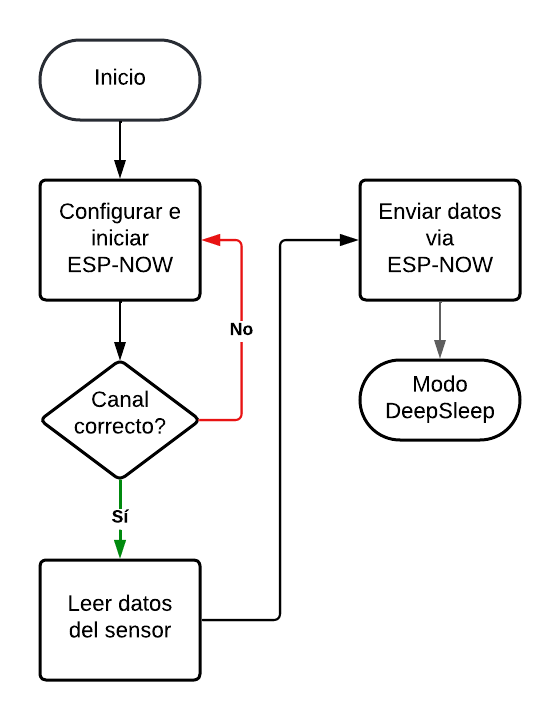
\includegraphics[width=0.5\textwidth]{./Figures/flujo_nodo_sensor.png}
\caption{Diagrama de flujo de los nodos sensores.}
\label{fig:flujoSensor}
\end{figure}

\subsubsection{Módulo relés}

El nodo encargado de los relés sigue un funcionamiento similar al de los nodos sensores en cuanto a la configuración inicial de ESP-NOW, por lo que no es necesario volver a detallar ese proceso. La principal diferencia radica en que, en lugar de tomar lecturas de un sensor, este nodo inicializa los relés y envía el estado en el que se encuentran al \textit{gateway}.

Una vez enviados los estados, el nodo queda a la espera de recibir instrucciones para modificar alguno de los relés. Si se recibe una solicitud para cambiar el estado de uno o más relés, el nodo ejecuta el cambio y, a continuación, envía nuevamente la información actualizada al \textit{gateway}.
Al igual que en los nodos sensores, la información se envía de forma encriptada para garantizar la seguridad de los datos transmitidos. De la misma manera, cualquier información que llega al nodo, como instrucciones para cambiar el estado de los relés, es desencriptada antes de ser procesada.

Este nodo no entra en \textit{modo DeepSleep}, ya que es necesario garantizar que los relés respondan de manera inmediata a cualquier instrucción de control que pueda recibirse.

En la figura \ref{fig:flujoRele} se puede observar el diagrama de flujo del módulo relés. 

\begin{figure}[H]
\centering 
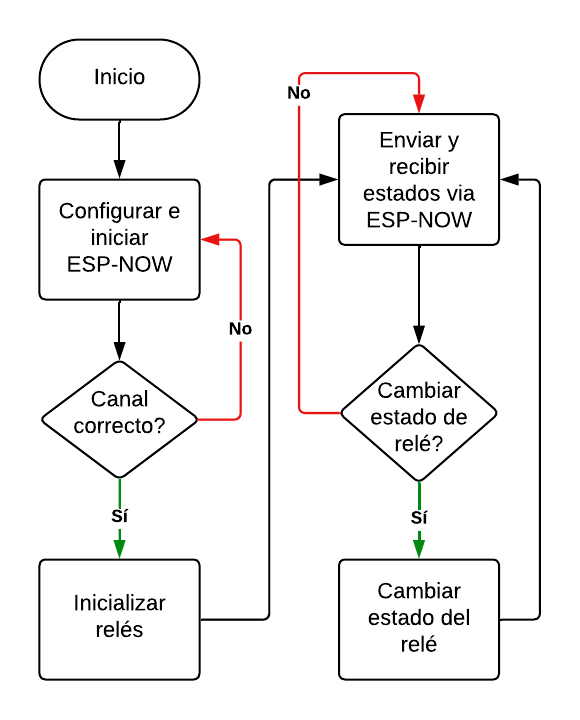
\includegraphics[width=0.5\textwidth]{./Figures/flujo_rele.png}
\caption{Diagrama de flujo del módulo relés.}
\label{fig:flujoRele}
\end{figure}

\subsection{Nodo Central}

El \textit{gateway} puede iniciar en dos modos diferentes: \textit{Modo Cliente} (CL) o \textit{Modo Access Point} (AP), dependiendo de la configuración cargada en el dispositivo. Una vez determinado el modo de operación, se configura e inicia la comunicación ESP-NOW en \textit{modo de difusión}.

\begin{itemize}
	\item Modo AP: en este caso, el \textit{gateway} actúa como un punto de acceso local, lo que significa que no está conectado a internet. Se inicia el servidor HTTP para proporcionar una interfaz web accesible a través de una red local, permitiendo al usuario monitorear y gestionar el sistema directamente sin necesidad de conexión externa.
	\item Modo CL: al iniciar en este modo significa que está conectado a internet a través de una red Wi-Fi. Se establece una conexión segura con un \textit{broker} MQTT. Para ello, se utilizan un nombre de usuario, una contraseña y certificados TLS para asegurar la comunicación. Además, el gateway se suscribe a un tópico específico del \textit{broker} MQTT, lo que le permite recibir mensajes relacionados con los sensores. Por último se inicia el servidor HTTP, lo que permite el acceso a la interfaz web embebida para monitorear y gestionar el sistema desde cualquier lugar con acceso a internet.
\end{itemize}

En la figura \ref{fig:flujoCentral} se puede observar el diagrama de flujo general del nodo central. 

\begin{figure}[H]
\centering 
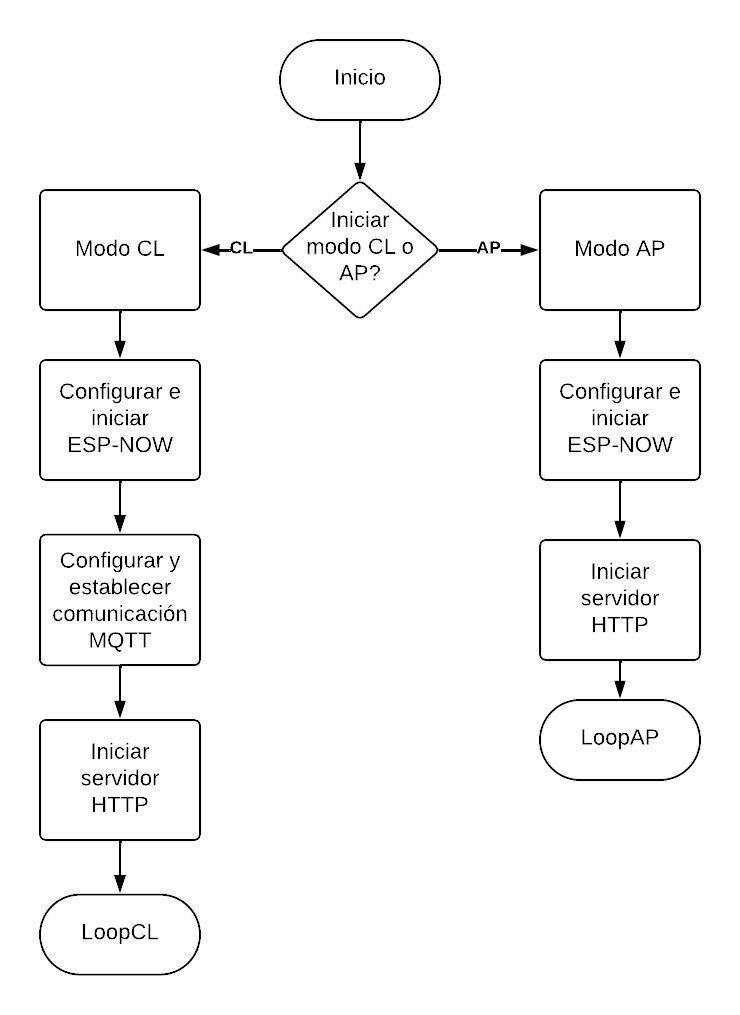
\includegraphics[width=0.7\textwidth]{./Figures/flujo_central.png}
\caption{Diagrama de flujo del nodo central.}
\label{fig:flujoCentral}
\end{figure}

\subsubsection{Loop AP}

En la figura \ref{fig:flujoAP} se puede observar el diagrama de flujo del loopAP. 

Una vez que el \textit{gateway} se ha iniciado en Modo AP y se ha configurado correctamente la comunicación ESP-NOW, entra en un bucle continuo de monitoreo y control, conocido como LoopAP. En este modo el \textit{gateway} realiza las siguientes acciones:

\begin{itemize}
	\item Monitoreo de nodos: el \textit{gateway} espera recibir datos de los nodos sensores y del módulo de relés a través de ESP-NOW. Al recibir información, ya sea de sensores o del estado de los relés, estos datos se envían y muestran en la PWA en tiempo real.
	\item Verificación de cambios en la PWA: si no se recibe información desde los nodos, el \textit{gateway} revisa si hubo un cambio en el estado de los relés en la PWA. Si detecta un cambio, envía la actualización al nodo correspondiente mediante ESP-NOW.
	\item Reinicio del ciclo: luego de procesar cualquier evento, el \textit{gateway} regresa al inicio del ciclo, quedando en espera de nuevos datos o cambios.
\end{itemize}


\begin{figure}[H]
\centering 
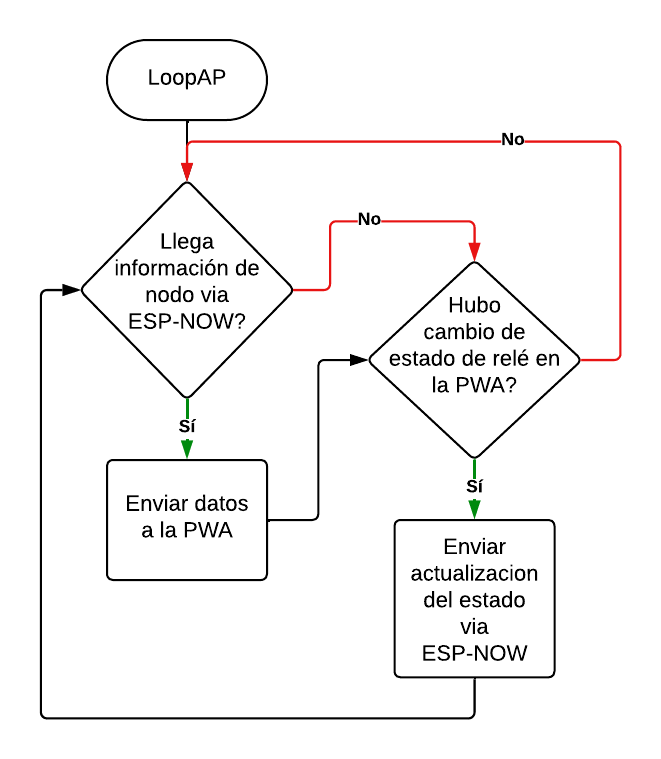
\includegraphics[width=0.5\textwidth]{./Figures/flujo_ap.png}
\caption{Diagrama de flujo del loop AP.}
\label{fig:flujoAP}
\end{figure}

\subsubsection{Loop CL}

En este modo, los datos de los sensores no solo se muestran localmente en la PWA, sino que también se publican en el \textit{broker} MQTT, lo que permite que sean almacenados y procesados remotamente. Esto garantiza una mayor capacidad de monitoreo y análisis.
Otra diferencia importante es la sincronización con el servidor IoT. Mientras que en el LoopAP los cambios en el estado de los relés solo se controlan desde la PWA, en el LoopCL también se monitorea si el estado de los relés ha sido modificado desde el servidor IoT. Esto posibilita la gestión remota de los dispositivos, permitiendo que el usuario controle y supervise el invernadero desde cualquier lugar con acceso a internet, una funcionalidad que no está disponible en el modo AP.

En la figura \ref{fig:flujoAP} se presenta el diagrama de flujo del loopCL. 

\begin{figure}[H]
\centering 
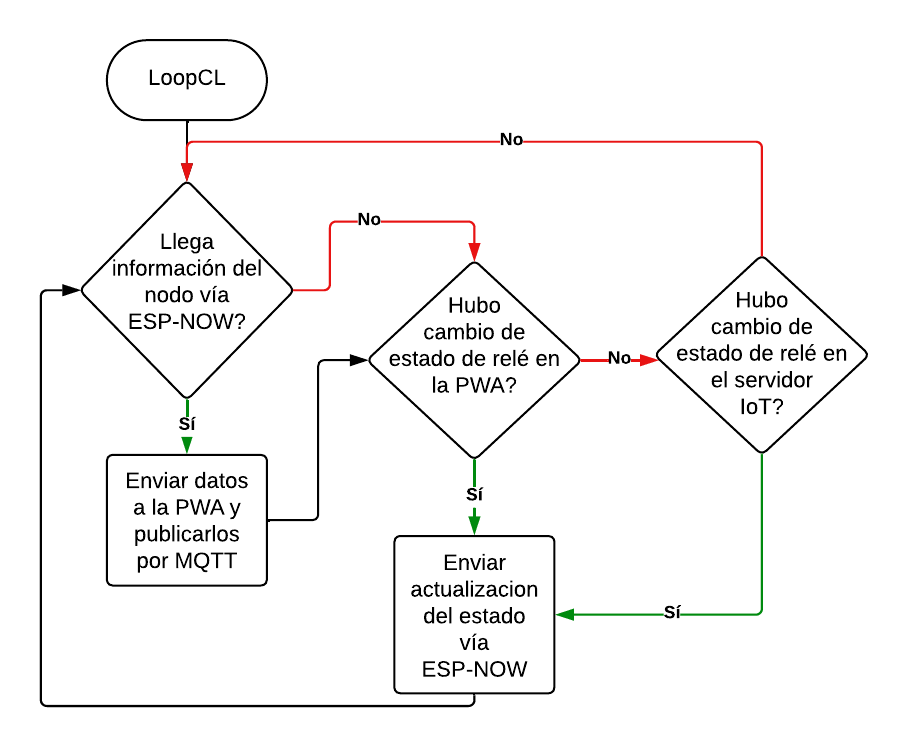
\includegraphics[width=0.6\textwidth]{./Figures/flujo_cl.png}
\caption{Diagrama de flujo del loop CL.}
\label{fig:flujoCL}
\end{figure}

%----------------------------------------------------------------------------------------
\section{Desarrollo de la aplicacion web progresiva}

La aplicación web progresiva (PWA) fue desarrollada utilizando tecnologías web estándar como HTML \citep{html}, CSS \citep{css} y JavaScript \citep{js}. Su objetivo principal es proporcionar a los usuarios una interfaz intuitiva y accesible para visualizar la información generada por los sensores y monitorear los estados de los relés. Además, la PWA permite a los usuarios interactuar con los relés, facilitando el cambio de estado de estos dispositivos en tiempo real. También se incluye la funcionalidad para editar la configuración del \textit{gateway}, ofreciendo un control integral y eficiente del sistema.

\subsection{Login de la PWA}

En la figura \ref{fig:login} se muestra la pantalla de inicio de sesión, donde el usuario debe ingresar su nombre de usuario y contraseña para acceder al sistema. 

\begin{figure}[H]
\centering 
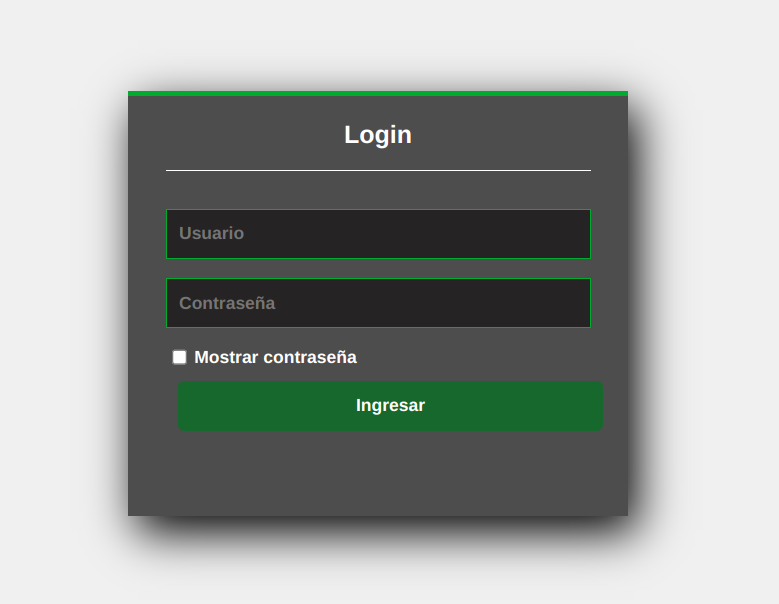
\includegraphics[width=0.7\textwidth]{./Figures/login.png}
\caption{Pantalla de login.}
\label{fig:login}
\end{figure}


El sistema cuenta con un método de validación basado en \textit{localstorage}, lo que garantiza que, incluso si se conoce la URL de acceso a las distintas pantallas, no se puede ingresar sin haber iniciado sesión previamente. 

En caso de que se cometa un error al ingresar las credenciales, el sistema desplegará un mensaje indicando que son incorrectas, tal como se muestra en la figura \ref{fig:login_inc}.


\begin{figure}[H]
\centering 
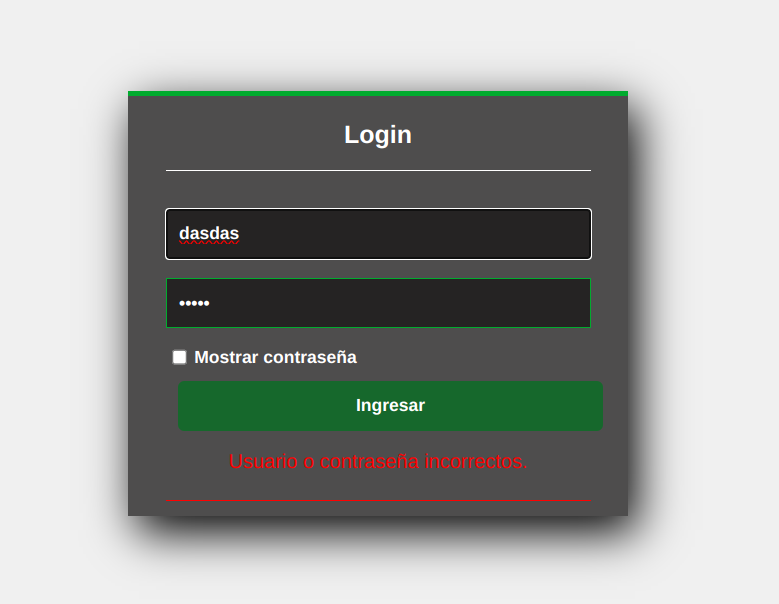
\includegraphics[width=0.7\textwidth]{./Figures/login_inc.png}
\caption{Pantalla de login con datos incorrectos.}
\label{fig:login_inc}
\end{figure}

\subsection{Pagina principal}

La figura \ref{fig:home_ini} muestra la pantalla principal de la aplicación web progresiva (PWA) sin ningún sensor ni relé cargado. En esta pantalla, los usuarios pueden acceder a dos funciones principales mediante botones ubicados en la parte superior derecha: uno para navegar a la página de configuración y otro para cerrar sesión. La página también está preparada para desplegar la información de los sensores y relés, que aparecerán en las secciones correspondientes una vez se carguen los datos.

\begin{figure}[H]
\centering 
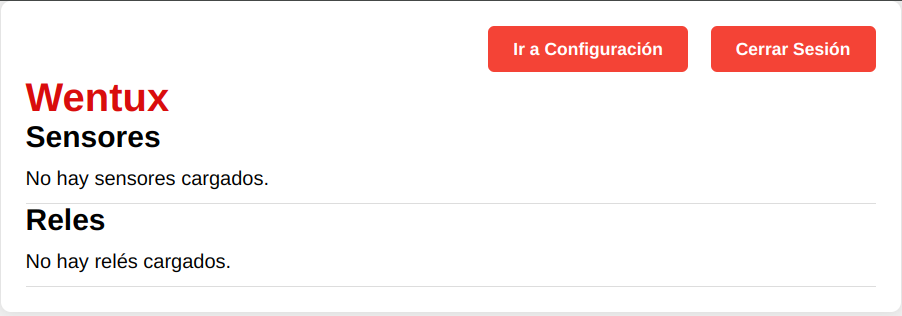
\includegraphics[width=0.8\textwidth]{./Figures/home_ini.png}
\caption{Pantalla principal.}
\label{fig:home_ini}
\end{figure}

En la figura \ref{fig:home_comp} se muestra la pantalla principal de la PWA con los sensores y relés ya cargados. En esta interfaz, los usuarios pueden visualizar en tiempo real la información de los sensores y los relés conectados al sistema.


\begin{figure}[H]
\centering 
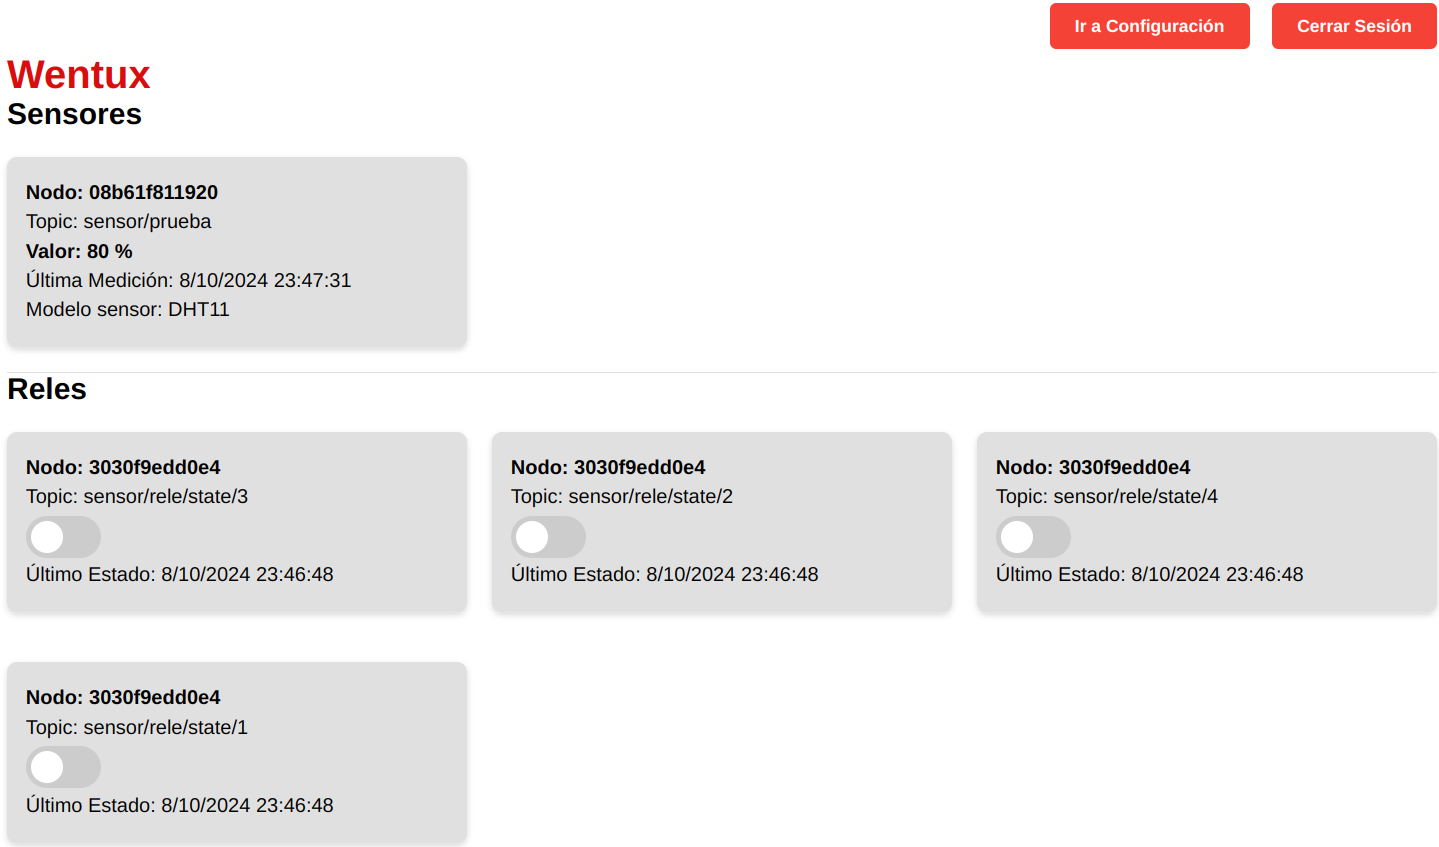
\includegraphics[width=1\textwidth]{./Figures/home_comp.png}
\caption{Pantalla principal.}
\label{fig:home_comp}
\end{figure}


Cada sensor presenta los siguientes atributos:

\begin{itemize}
	\item Nodo: este campo muestra la dirección MAC del nodo al que está conectado el sensor.
	\item Topic: define la variable que está siendo medida por el sensor. Puede variar según el tipo de sensor, por ejemplo, sensor/temp para la temperatura, sensor/hum para la humedad, o sensor/co2 para la concentración de CO2, entre otros.
	\item Valor: indica el valor actual de la variable que el sensor está midiendo.
	\item Última medición: muestra la fecha y hora de la última vez que se recibió un dato válido desde el sensor.
	\item Modelo sensor: especifica el nombre o tipo del sensor utilizado.
\end{itemize}

En la sección de relés, la PWA permite a los usuarios interactuar y controlar los dispositivos conectados:

\begin{itemize}
	\item Nodo: al igual que los sensores, este campo muestra la dirección MAC del nodo al que está asociado el relé.
	\item Topic: define el relé específico que se está controlando, utilizando un formato del tipo sensor/rele/state/X, donde X representa el número del relé.
	\item Botón on/off: cada relé tiene un interruptor visual que permite al usuario encender o apagar el dispositivo manualmente.
	\item Último estado: registra la fecha y hora del último cambio en el estado del relé.
\end{itemize}

\subsection{Pantalla de configuración}

La página de configuración permite al usuario ajustar los parámetros clave del sistema para su correcto funcionamiento en diferentes modos operativos, dependiendo de si el dispositivo actúa como Cliente (CL) o como Punto de Acceso (AP). La configuración se realiza a través de un formulario con varios campos que permiten personalizar aspectos como la conexión Wi-Fi, el broker MQTT, y otros detalles del sistema embebido.

En las figuras \ref{fig:config_1} y \ref{fig:config_2} se puede observar la pantalla de configuración donde tenemos:

Modos de Operación:

\begin{itemize}
	\item Cliente (CL): en este modo, el dispositivo se conecta a una red Wi-Fi externa.
	\item Punto de Acceso (AP): en este modo, el dispositivo no tiene acceso a Internet.
\end{itemize}

Campos principales:

\begin{itemize}
	\item SSID y Contraseña: estos campos permiten configurar la red Wi-Fi a la que se conectará el dispositivo en modo Cliente. 
	\item SSID y Contraseña del AP: estos datos se utilizan cuando el dispositivo está en modo Punto de Acceso, permitiendo a otros dispositivos conectarse directamente a este.
	\item Cliente ID, MQTT \textit{Broker}, Usuario y Contraseña MQTT: son los parámetros necesarios para configurar la comunicación con el servidor de MQTT, que es fundamental para transmitir los datos de los sensores y controlar los relés remotamente.
	\item Puerto: especifica el puerto utilizado para la conexión MQTT.
\end{itemize}

Configuración de Fecha y Hora:

\begin{itemize}
	\item cuando el dispositivo está en modo Cliente sincroniza automáticamente la fecha y la hora a través de Internet, por lo que los campos de Fecha y Hora en la página de configuración están deshabilitados.
	\item Cuando el dispositivo está en modo AP, es necesario ingresar manualmente la fecha y la hora para asegurar que el sistema embebido, que no tiene acceso a Internet, opere en el tiempo correcto.
\end{itemize}


Botones:
\begin{itemize}
	\item Guardar Configuración: este botón guarda los cambios realizados en los parámetros del sistema. Al hacer clic, se edita el archivo de configuración en el sistema y luego se reinicia el dispositivo para aplicar los nuevos parámetros. Este reinicio asegura que el sistema funcione con la configuración más reciente sin necesidad de intervención manual adicional.
	\item Volver a Inicio: este botón redirige al usuario de vuelta a la pantalla principal de la aplicación, donde puede visualizar los datos de los sensores y relés configurados en el sistema.
\end{itemize}

Con esta configuración flexible, el sistema puede adaptarse tanto a escenarios con conexión a Internet como a entornos sin conectividad, lo que lo hace ideal para ser implementado en diversos contextos, como invernaderos o áreas rurales donde la conectividad puede ser limitada.


\begin{figure}[H]
\centering 
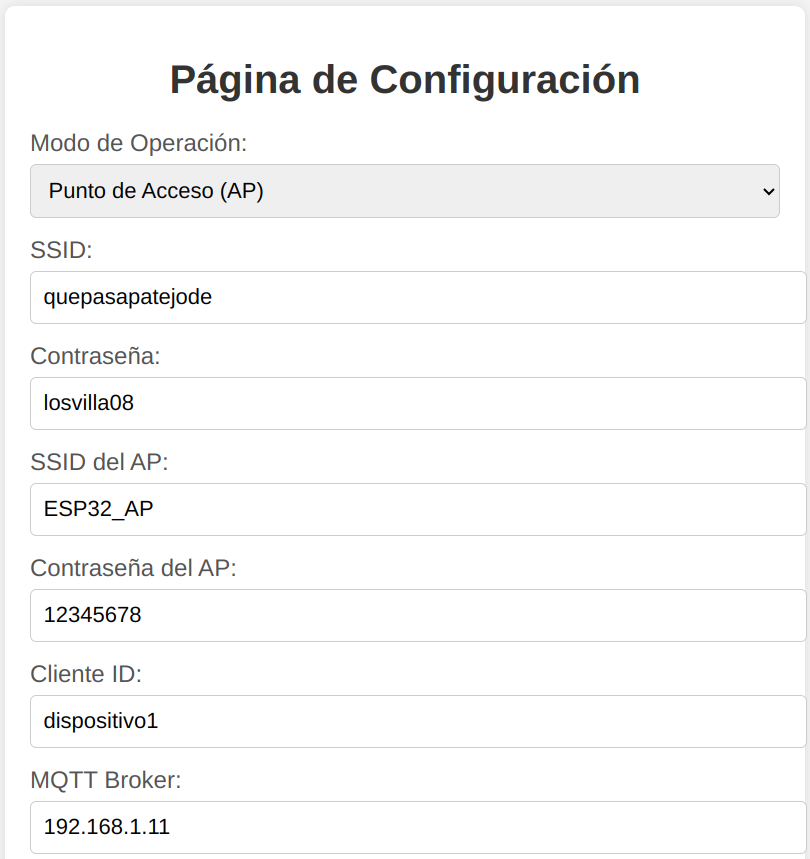
\includegraphics[width=0.8\textwidth]{./Figures/config_1.png}
\caption{Pantalla de configuración.}
\label{fig:config_1}
\end{figure}


\begin{figure}[H]
\centering 
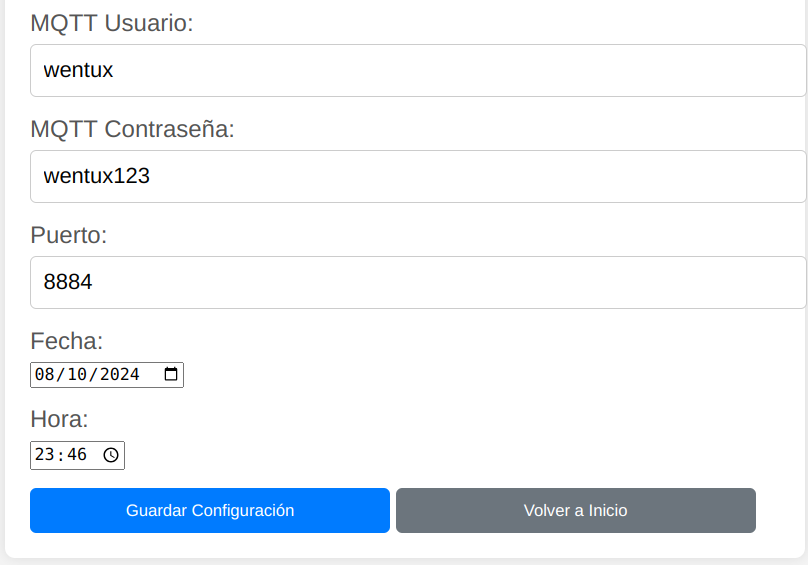
\includegraphics[width=0.8\textwidth]{./Figures/config_2.png}
\caption{Pantalla de configuración.}
\label{fig:config_2}
\end{figure}





%----------------------------------------------------------------------------------------
\section{Implementación del servidor IoT}


Para la implementación del servidor IoT se utilizó OpenRemote, el cual se despliega de manera local mediante el uso de Docker \citep{docker}. Docker permite levantar de forma rápida y eficiente el entorno del servidor, facilitando la gestión de contenedores y asegurando que todo el sistema funcione de manera óptima y sin conflictos de dependencias. Este enfoque permite que el servidor esté operativo de manera ágil y estandarizada, sin la necesidad de configuraciones manuales complejas.

Se explicará el proceso de inicio de sesión, la configuración del agente MQTT para conectar con el broker, la creación y configuración de los objetos correspondientes a los sensores y relés mediante Thing Asset, la definición y uso de reglas para automatizar acciones y, finalmente, la configuración del dashboard para la visualización de los datos.


\subsection{Login}

En la figura \ref{fig:login_op} se presenta la pantalla de inicio de sesión, donde el usuario debe ingresar su nombre de usuario o correo electrónico, junto con la contraseña, para acceder al sistema. Si las credenciales ingresadas son incorrectas, el sistema mostrará un mensaje de advertencia indicando el error, como se ilustra en la figura \ref{fig:login_op_inc}

\begin{figure}[H]
\centering 
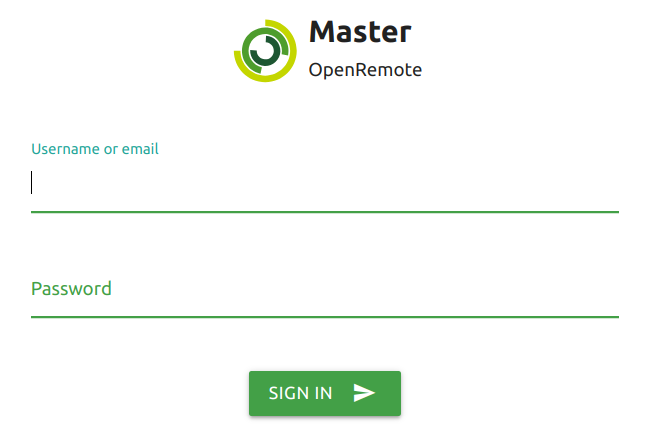
\includegraphics[width=0.7\textwidth]{./Figures/login_op.png}
\caption{Pantalla de login de OpenRemote.}
\label{fig:login_op}
\end{figure}

\begin{figure}[H]
\centering 
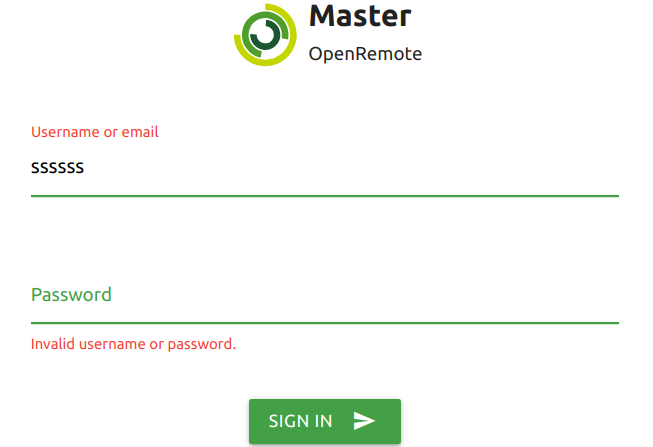
\includegraphics[width=0.7\textwidth]{./Figures/login_op_inc.png}
\caption{Pantalla de login de OpenRemote con datos incorrectos.}
\label{fig:login_op_inc}
\end{figure}    

\subsection{Agente MQTT y activos}
Se explicará cómo usar el Agente MQTT en OpenRemote y cómo utilizar los activos (assets) para gestionar la información de los sensores y relés a través de la plataforma.

\subsubsection{Agente MQTT}

OpenRemote cuenta con un Agente MQTT (Cliente) que permite conectar el servidor a un broker MQTT externo. Para establecer esta conexión, es necesario configurar el host del broker, el Cliente ID, el puerto de conexión, así como las credenciales de acceso, que incluyen el usuario y la contraseña. Una vez configurados estos parámetros, el agente se encarga de gestionar los datos que se transmiten entre los sensores y el servidor. Esta integración garantiza que la información fluya de manera eficiente y pueda ser utilizada para la visualización y control de dispositivos a través de la plataforma.

En la figura \ref{fig:conf_mqtt} se puede observar la pantalla de configuración del agente mqtt.

\begin{figure}[H]
\centering 
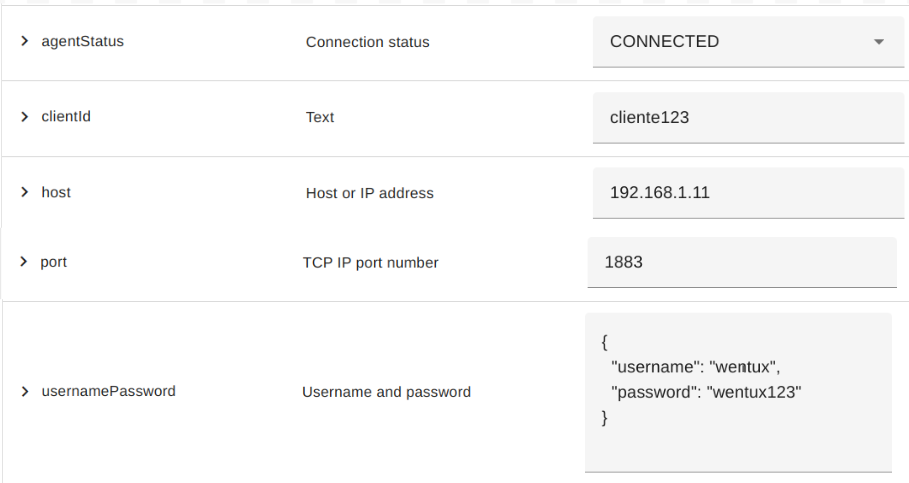
\includegraphics[width=0.9\textwidth]{./Figures/conf_mqtt.png}
\caption{Configuración del agente mqtt.}
\label{fig:conf_mqtt}
\end{figure}

\subsubsection{Activos (Assets)}

En OpenRemote, los activos representan los objetos correspondientes a los sensores y relés del sistema. Cada activo contiene atributos que reflejan diferentes tipos de datos, como valores de temperatura, humedad o estado de los relés. Para vincular estos atributos al agente MQTT, se utiliza la opción de Agent Link, que permite asociar un atributo a un tópico específico de publicación o suscripción en el broker MQTT, asegurando que los datos recibidos o enviados se manejen correctamente. Esta configuración facilita la integración de los dispositivos físicos con el sistema de gestión IoT. Esto se ilustra en la figura \ref{fig:activo_conf}, donde se muestra el nombre del activo, que en este caso es 'Rele', y su tipo, que es 'boolean'.

\begin{figure}[H]
\centering 
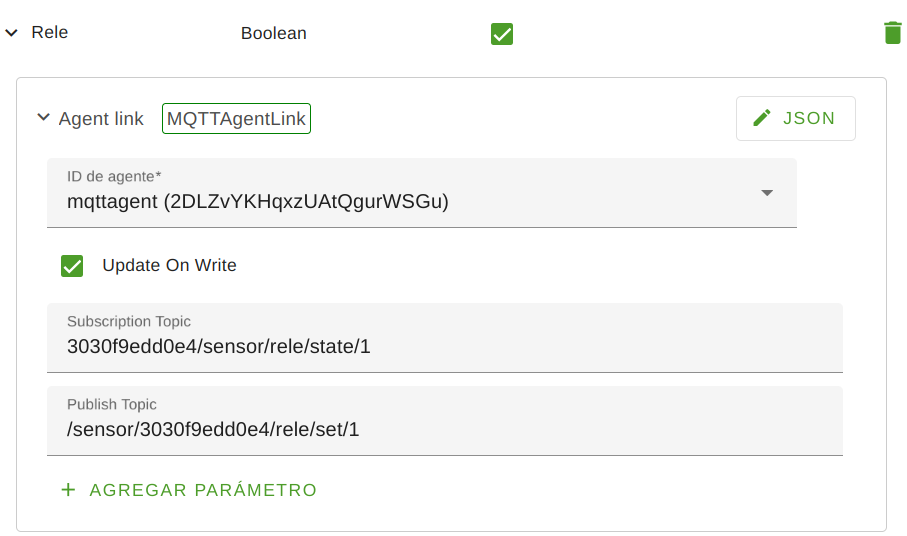
\includegraphics[width=0.9\textwidth]{./Figures/activo_conf.png}
\caption{Configuración del activo.}
\label{fig:activo_conf}
\end{figure}

En la figura \ref{fig:activo_prin} se muestra la pantalla principal de los activos. En la parte izquierda se puede observar el \textit{mqttagent} junto con los activos asociados. También se presenta la información del sensor 1, donde los campos de notas y posición están incorporados al activo por defecto y no pueden deshabilitarse. Se han agregado los atributos 'rele', 'rele 2' y 'temp', que están suscritos al broker MQTT para recibir información. En el caso de los relés, son checkboxes que funcionan con lógica booleana y pueden publicar su estado en caso de que cambien manualmente o a través de reglas.

\begin{figure}[H]
\centering 
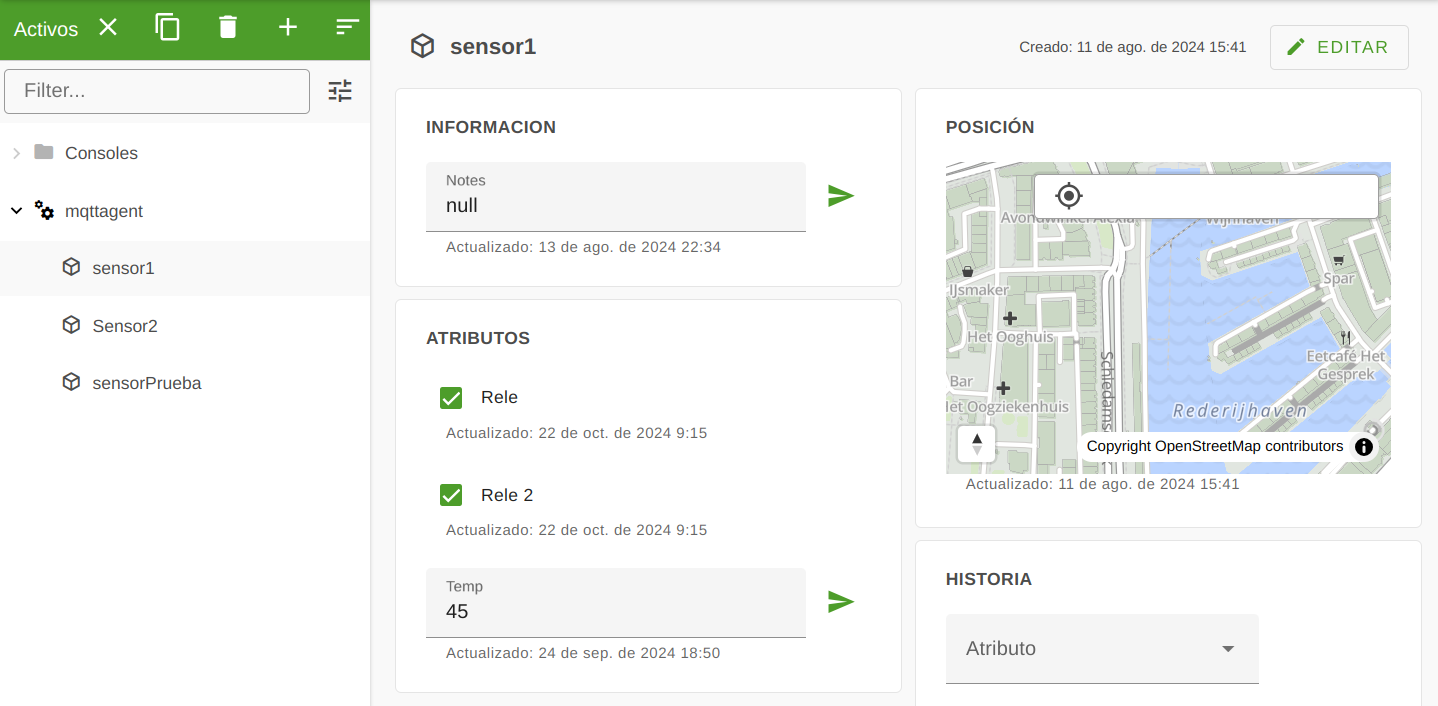
\includegraphics[width=1\textwidth]{./Figures/activo_prin.png}
\caption{Pantalla principal de los activos.}
\label{fig:activo_prin}
\end{figure}        


\subsection{Reglas}

OpenRemote incluye un motor de reglas que permite a los usuarios automatizar tareas de diversas maneras. Un tipo de regla que destaca es la regla 'Cuando-Entonces', que facilita la creación de acciones basadas en eventos de forma sencilla.

Con las reglas 'Cuando-Entonces', podemos establecer una condición que, al cumplirse, activa una acción. Por ejemplo, en la figura \ref{fig:reglas}, se muestra el activo sensor1, donde si el atributo 'temp' supera los 40 grados, entonces el relé del activo sensor1 se activa mientras que el relé 2 se apaga.

\begin{figure}[H]
\centering 
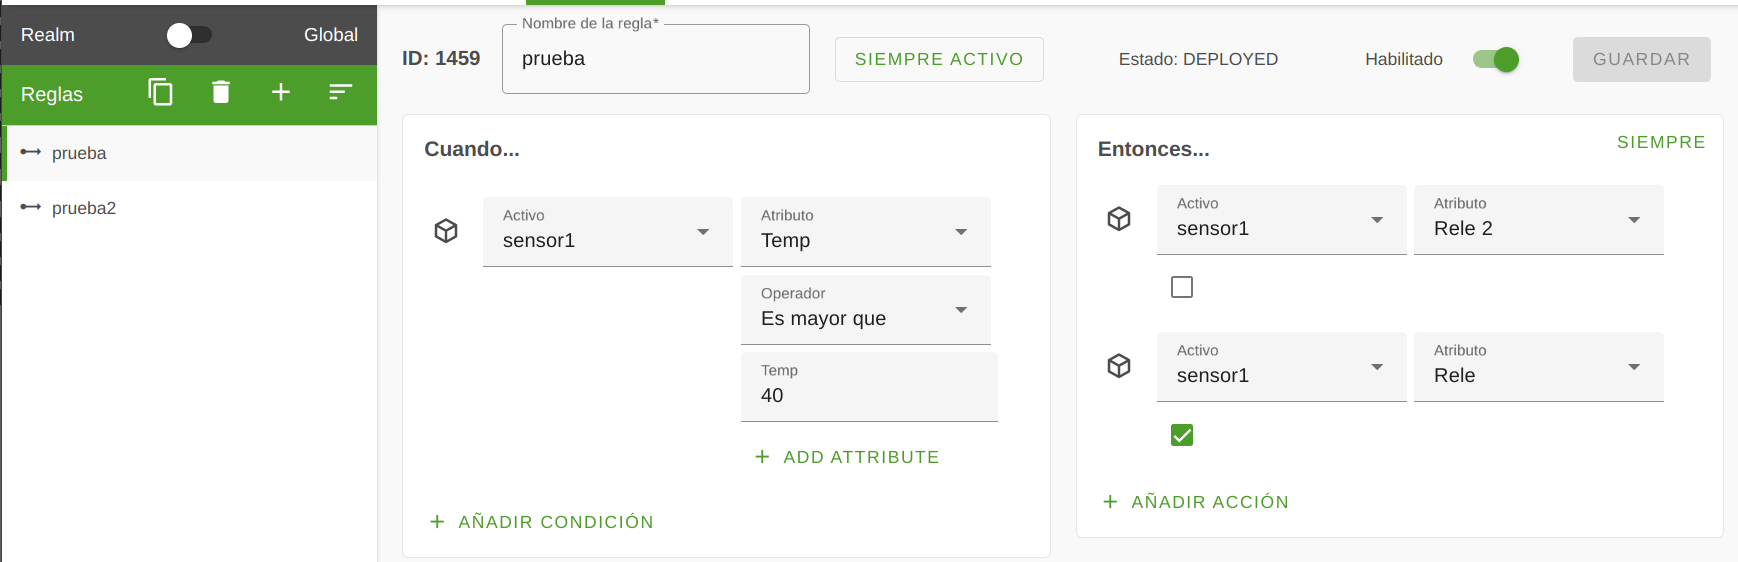
\includegraphics[width=1\textwidth]{./Figures/reglas.png}
\caption{Pantalla principal de las reglas.}
\label{fig:reglas}
\end{figure}      

\subsection{Dashboard}

OpenRemote ofrece una funcionalidad de \textit{dashboard} totalmente configurable, que permite a los usuarios visualizar los datos de sus sensores y dispositivos de manera gráfica y sencilla. Este panel puede personalizarse utilizando diversos widgets según las necesidades del trabajo. En la figura \ref{fig:dashboard} se muestra un ejemplo de \textit{dashboard} donde se ha configurado un gráfico de líneas para monitorear la temperatura registrada por un sensor, así como la visualización del estado de dos relés. Esta flexibilidad en la configuración permite adaptar la interfaz a distintos casos de uso, ofreciendo una solución visual intuitiva para la monitorización y el control de dispositivos.

\begin{figure}[H]
\centering 
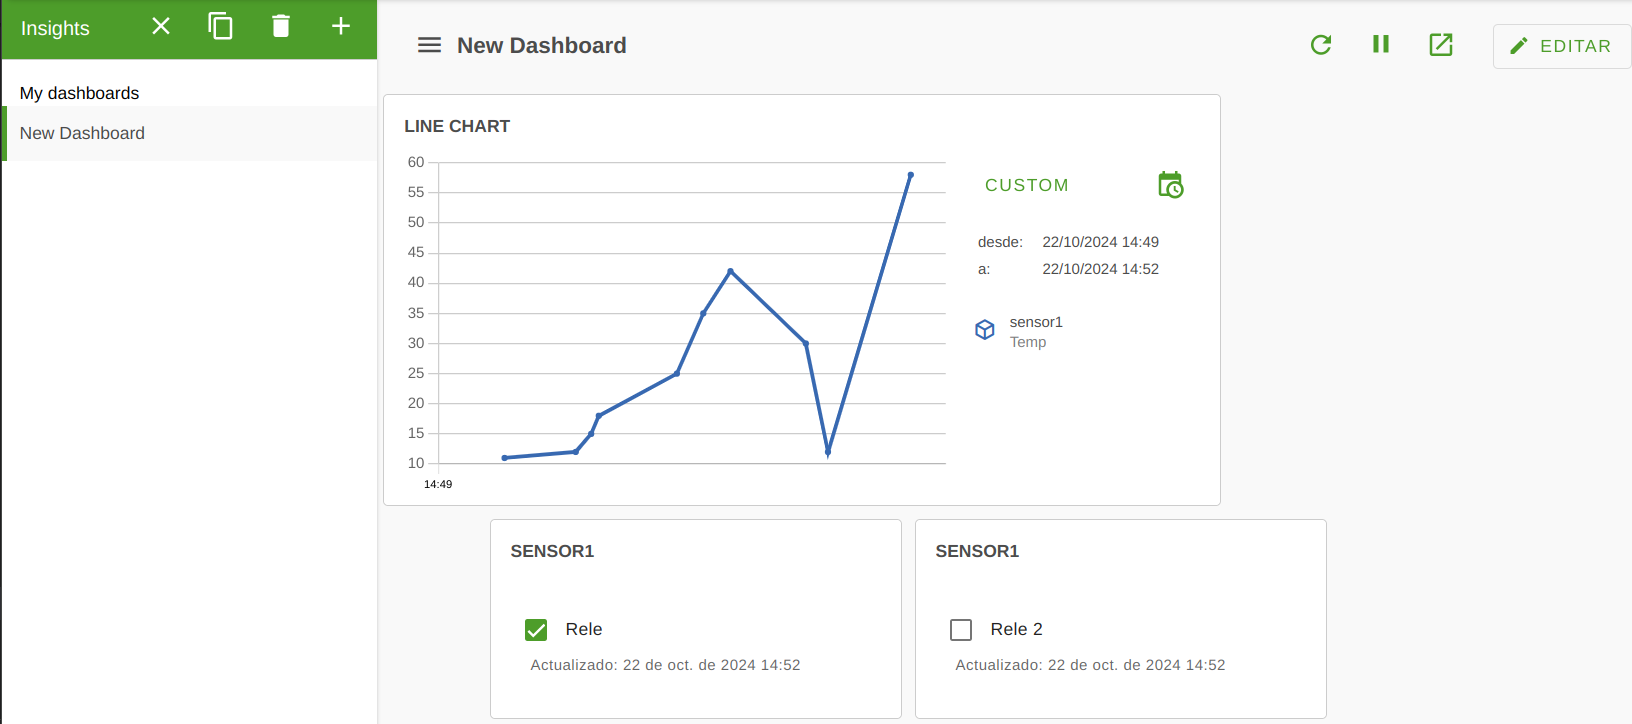
\includegraphics[width=1\textwidth]{./Figures/dashboard.png}
\caption{Pantalla principal del dashboard.}
\label{fig:dashboard}
\end{figure} 


%----------------------------------------------------------------------------------------